\documentclass[12pt]{article} 
\usepackage{amsmath} 
\usepackage{amsfonts}
\usepackage{amssymb} 
\usepackage[utf8]{inputenc} 
\usepackage[T1,T2A]{fontenc}
\usepackage[english, russian]{babel} 
\usepackage{graphicx}
\usepackage{float}
\usepackage[left=2cm,right=2cm,top=2cm,bottom=2cm]{geometry}
\usepackage{wrapfig}
\usepackage{pgfplots} 
\usepackage{setspace} 
\usepackage{indentfirst}
\usepackage{subfigure} 
\usepackage{hyperref}

\graphicspath{{pictures}}

\title{ 
Лабораторная работа 2.5.1 \\
<<Измерение коэффициента поверхностного натяжения жидкости>>
}

\author{Балдин Виктор, Б01-303}

\begin{document}
    \maketitle
    \paragraph{Цель работы}
    \begin{enumerate}
        \item Измерение коэффициента поверхностного натяжения исследуемой 
        жидкости при разных температурах.
        \item Определение полной поверхностной энергии и теплоты, необходимой
        для изотермического образования единицы поверхности жидкости.
    \end{enumerate}
    \paragraph{Оборудование}
    Прибор Ребиндера с термостатом; исследуемые жидкости; стаканы.
    
    \section{Теоретическая часть}
    Наличие поверхностного слоя приводит к различию давлений по разные стороны
    от искривлённой границы раздела двух сред. Для сферического пузырька внутри
    жидкости избыточное давление даётся формулой Лапласа (5.15):
    $$ \Delta P=P_{\text {внутри }}-P_{\text {Снаружи }}=\frac{2 \sigma}{r} .  $$

    Эта формула лежит в основе предлагаемого метода определения коэффициента
    поверхностного натяжения жидкости. Измеряется давление, необходимое для
    выталкивания в жидкость пузырька газа.

    \section{Экспериментальная установка}
    Исследуемая жидкость (анилин) наливается в сосуд В.
    Дистиллированная вода наливается в сосуд Е. Сосуды закрыты пробками. Через
    пробку сосуда, в котором проводятся измерения, проходит полая металлическая игла
    С, нижний конец которой погружен в жидкость, а верхний открыт в атмосферу. Если
    другой сосуд герметично закрыт, то в сосуде с иглой создается разрежение,
    и пузырьки воздуха начинают пробулькивать через жидкость через жидкость.
    
    \begin{figure}[H]
        \centering
        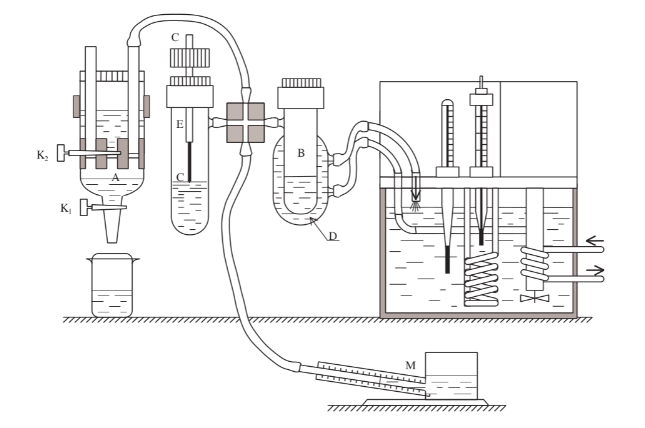
\includegraphics[scale=2]{stand.png}
        \caption{
        Схема установки для измерения температурной зависимости 
        коэффициента поверхностного натяжения
        }
    \end{figure} 
    Для стабилизации температуры исследуемой жидкости через рубашку D непрерывно
    прогоняется вода из термостата.

    Обычно кончик иглы лишь касаёется поверхности жидкости, чтобы исключить
    влияние гидростатического давления столба жидкости. Однако при измерении
    температурной зависимости коэффициента поверхностного натяжения возникает
    ряд сложностей. Во-первых, большая теплопроводность металлической трубки
    приводит к тому, что температура на конце трубки заметно ниже, чем в глубине
    жидкости. Вовторых, тепловое расширение поднимает уровень жидкости при
    увеличении температуры. Это гидростатическое давление вычитается из падения
    лапласова давления вследствие уменьшения $\sigma$, и в опыте с анилином,
    например, наблюдаемый эффект меняет знак при высоте столба жидкости порядка
    пяти сантиметров.
    
    Обе погрешности можно устранить, погрузив кончик трубки до самого дна.
    Полное давление, измеренное при этом микроманометром, $P=\Delta P+\rho g h$.
    Заметим, что $\rho g h$ от температуры практически не зависит, так как
    подъём уровня жидкости компенсируется уменьшением её плотности (произведение
    $\rho h$ определяется массой всей жидкости и поэтому постоянно). Величину
    $\rho g h$ следует измерить экспериментально двумя методами. Во-первых, 
    замерить величину $\Delta P_1 = \Delta P'$, когда кончик трубки только
    касается поверхности жидкости. Затем при этой же температуре опустить иглу
    до дна и замерять $P_2 = \rho gh + \Delta P''$. Из-за несжимаемости 
    жидкости можно положить $\Delta P' = \Delta P''$ и тогда $\rho gh = P_2 -
    P_1$. Во-вторых, при измерениях $P_1$ и $P_2$ замерить линейкой глубину
    погружения иглы $h_1$ и $h_2$. Это легко сделать, замеряя расстояние 
    между верхним концом иглы и любой неподвижной частью прибора.

    \section{Ход работы}

\end{document}
